\title{Orthogonal Compliments}
\subtitle{\SubTitleName}
\institute[]{\Course}
\author{\Instructor}
\maketitle   
  


\frame{\frametitle{Topics and Objectives}
\Emph{Topics} \\
%\TopicStatement
\begin{itemize}

    % \item dot products

    % \item magnitude of vectors
    
    % \item distances in $\mathbb R^n$ 
    
    % \item angles between vectors

    % \item orthogonal vectors and dot products
    
    \item orthogonal compliments
    

\end{itemize}

\vspace{0.5cm}

\Emph{Learning Objectives}\\

\LearningObjectiveStatement

\begin{itemize}

    % \item characterize relationships between vectors using the (a) dot product of two vectors, (b) length (or magnitude) of a vector, (c) distance between points in $ \mathbb R^n$, and (d) angles between vectors
    
    \item apply theorems related to orthogonality to characterize vectors and subspaces
    
\end{itemize}

} 




\begin{frame}[t]\frametitle{Orthogonal Compliments} 

\vspace{-10pt} 

\begin{center}\begin{tikzpicture} \node [mybox](box){\begin{minipage}{0.95\textwidth}

\vspace{2pt} 

    Let $W$ be a subspace of $\mathbb R ^{n}$.  Vector $\vec z \in \mathbb R ^{n}$ is \Emph{orthogonal} to $W$ if $\vec z$ is orthogonal to every vector in $W$.

    \vspace{12pt} 

    The set of all vectors orthogonal to $ W$ is a subspace, the \Emph{orthogonal compliment} of $W$, or $ W ^{\perp}$.
    \begin{equation*}
        W ^{\perp} = \{ \vec z \in \mathbb R ^{n}  \;:\;  \vec z \cdot  \vec w = 0 \ \text{for all } \vec w \in W \} 
    \end{equation*}

\end{minipage}};
\node[fancytitle, right=10pt] at (box.north west) {Definitions};
\end{tikzpicture}\end{center}

\end{frame}









\begin{frame}\frametitle{Example: $(\text{Col} A)^{\perp}$} 


\begin{columns}
\begin{column}{0.5\textwidth}
   Suppose $A = \spalignmat{1 3;2 6}$. 
   \begin{itemize}
       \item<2-> $\text{Col} A$ is the span of $\vec a_1 = \spalignmat{1;2}$  
       \item<3-> $(\text{Col} A )^{\perp}$ is the span of $\vec z = \spalignmat{2;-1}$
   \end{itemize}\end{column}\begin{column}{0.5\textwidth}  \vspace{-1cm} \begin{center}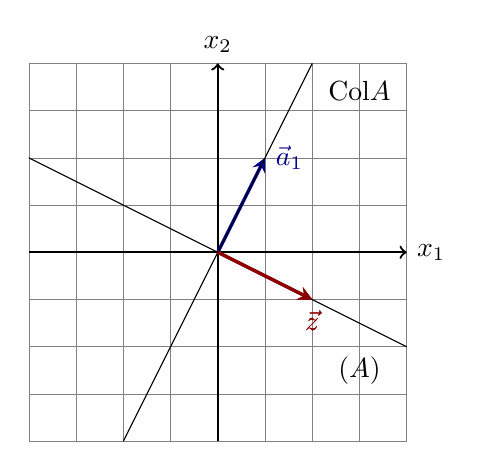
\begin{tikzpicture}
   [scale=.6,
   vectorblue/.style={-stealth,DarkBlue,very thick},
   vectorred/.style={-stealth,DarkRed,very thick}]
   \onslide<4->{
        \draw[help lines] (-4, -4) grid (4, 4);
        \draw[thick, ->] (-4, 0) -- (4, 0) node[anchor=west] {$x_1$};
        \draw[thick, ->] (0, -4) -- (0, 4) node[anchor=south] {$x_2$};
    }
    \onslide<5->{
        \draw[vectorblue]   (0,0) -- (1,2) node[anchor=west]{$\vec a_1$};
    }
    \onslide<6->{
        \node[overlay, above] at (3, 3) {Col$A$};
        \draw[-] (-2,-4) -- (2,4);
    }
    \onslide<7->{
        \draw[vectorred]   (0,0) -- (2,-1) node[anchor= north]{$\vec z$};
    }
    \onslide<8->{
        \node[overlay, below] at (3, -2) {$(\Col A)\Perp$};
        \draw[-] (-4,2) -- (4,-2);
        \draw[vectorred]   (0,0) -- (2,-1) node[anchor= north]{$\vec z$};
    }    
    \end{tikzpicture}
    \end{center}
\end{column}
\end{columns}


\end{frame}



\begin{frame}\frametitle{Example: $(\text{Nul} A)^{\perp}$} 

For $A = \spalignmat{1 3;2 6}$, sketch Nul$A$ and (Nul$A)^{\perp}$ on the grid below. 

\begin{center}
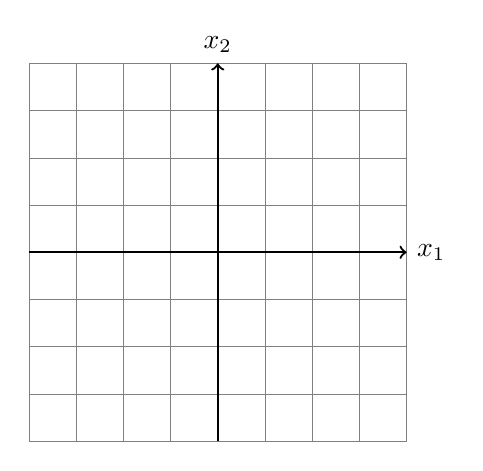
\begin{tikzpicture}
   [scale=.6,
   vectorblue/.style={-stealth,DarkBlue,very thick},
   vectorred/.style={-stealth,DarkRed,very thick}]
    \draw[help lines] (-4, -4) grid (4, 4);
    \draw[thick, ->] (-4, 0) -- (4, 0) node[anchor=west] {$x_1$};
    \draw[thick, ->] (0, -4) -- (0, 4) node[anchor=south] {$x_2$};
    \end{tikzpicture}
    \end{center}

\end{frame}









\begin{frame}\frametitle{Example: Equation of a Plane} 

    Line $L$ is a subspace of $\R^3$ spanned by $\vec v = \spalignmat{1;-1;2}$. Then the space $ L^{\perp}$ is a plane. Construct an equation of the plane $ L ^{\perp}$. 
    
    \vspace{6pt}

    \tdplotsetmaincoords{80}{100}
        \begin{tikzpicture}[
        scale=1.4,
        tdplot_main_coords,
        line/.style={DarkRed},
        vector/.style={-stealth,DarkBlue,very thick},
        vector guide/.style={dashed,gray}
        ]
        
            \coordinate (P) at (2,-1,2);  
            \coordinate (Q) at (2.4,-1.2,2.4);
            \coordinate (R) at (-1.2,.6,-1.2);
            \coordinate (O) at (0,0,0);
            
            % Draw Axes
            \draw[thick,->] (O) -- (2.8,0,0) node[anchor=north east]{$x$};
            \draw[thick,->] (0,-2,0) -- (0,2,0) node[anchor=north west]{$y$};
            \draw[thick,->] (O) -- (0,0,2) node[anchor=south]{$z$};            
            
            % Draw Plane (assume instructor will annotate slide with OneNote)
%            \filldraw[
%                draw=DarkBlue,% color of edge
%                fill=DarkBlue!20,% color of fill
%                opacity=.6, % sets opacity of fill and of edges
%            ]          
%            (-1,-1,0)
%            -- (1,1,0)
%            -- (-1,1,0)
%            -- (-3,-1,0)            
%            -- cycle;
  
            % Draw Vector and Line L
            \draw[line]     (R) -- (Q) node[anchor=north east]{$L$};
            \draw[vector]   (O) -- (P) node[anchor=north east]{$\vec v$};

            % Draw vector guides
            \draw[vector guide] (2,-1,0) -- (2,0,0) node[anchor= west]{$1$};      
            \draw[vector guide] (2,-1,0) -- (0,-1,0) node[anchor=south west]{$-1$};      
            \draw[vector guide] (2,-1,0) -- (2,-1,2);      
            
        \end{tikzpicture}
    
    % \begin{center} {\small Can also visualise line and plane with CalcPlot3D: \underline{web.monroecc.edu/calcNSF}} \end{center}

\end{frame}













    
    
    
\frame{\frametitle{Summary}

    \SummaryLine \vspace{4pt}
    \begin{itemize}\setlength{\itemsep}{8pt}

        \item orthogonal vectors and dot products
        
        \item orthogonal compliments
        
    \end{itemize}
    
    \vspace{8pt}
    \onslide<2->{A key concept in this video was that if $W$ is a subspace of $\mathbb R^n$, the \Emph{orthogonal compliment} of that subspace, or $W\Perp$, is the set of all vectors orthogonal to the vectors in $W$. }
}


